\subsubsection{Marine Geochemistry}
\index{Koschinsky, Andrea}

\paragraph{Research Team}
Andrea Koschinsky (Professor), Herwig Marbler (Post-doc),
Thomas Schirmer (Post-doc), Jule Mawick (lab technician), Daniela
Mei\ss ner (lab technician), Katja Schmidt (PhD Student), Cristiane Jost
(DAAD exchange PhD student), Aryani Sumoondur (MSc student), Prasesh
Sharma (MSc student) \\

The research activity in the field of marine geochemistry continued in
2006 with its focus on marine hydrothermal systems as part of the DFG
Special Priority program SPP 1144: \quotedblbase{}From Mantle to
Ocean: Energy-, Material- and Life Cycles at Spreading Axes``. The
objective of the priority program is to quantify the processes at the
mid-ocean ridges from geological and biological investigations. The
target areas of this program are the Mid-Atlantic Ridge (MAR) at 15$^\circ$N
and 4$^\circ$-11$^\circ$S. The project of the IUB geochemistry group is entitled
\quotedblbase{}Hydrothermal Fluids at the Mid-Atlantic Ridge as Media
for the Transport of Energy and Mass from the Crust into the Hydro-
and Biosphere``. The second 2-years term of this project has started
in October 2005.

Apart from the hydrothermal research, our activities on experimental
and theoretical investigations of interactions between dissolved
metals, mineral phases and biota in the marine systems were
continued. New activities in the field of marine mineral resources
have been started.

\paragraph{Highlights}
The highlight of the hydrothermal research was cruise M68/1 with R/V
Meteor, where A. Koschinsky was chief scientist. This cruise continued
exploration for hydrothermal fields on the southern Mid-Atlantic
Ridge, which had been started as part of the SPP 1144 in 2005. Besides
the revisit of hydrothermal fields discovered the year before, the
combined use of an autonomous underwater vehicle AUV ABE from the
Woods Hole Oceanographic Institution and the remotely operated vehicle
ROV Quest from Marum, Univ. Bremen enabled the discovery of another 8
hydrothermally active sites in the area between 4 and
10$^\circ$S. Temperature measurements of fluids in the young volcanic
system at 5$^\circ$S revealed the highest temperature ever measured so
far in a hydrothermal fluid: 407$^\circ$C. At 3000 m, the water depth
of the vent site, this point represents the so-called critical point
of seawater, which separates the subcritical from the supercritical
fluid range. Gas bubbles and depleted salinity indicate ``boiling''
and phase separation. While this system is clearly characterized by
subsurface leaching of basaltic rock, the newly discovered site at
8$^\circ$S shows clear signatures of mantle rocks, underlining the
importance of ultramafic-hosted (mantle-rock hosted) hydrothermal
systems on slow spreading ridges such as the Mid-Atlantic Ridge.

Further investigation of organic metal complexation in hydrothermal
fluids confirmed our preliminary data, that toxic metals such as
copper are largely controlled by binding to organic ligands. This
probably makes them less bioavailable. Metal analyses of organic
tissue of hydrothermal mussels are carried out to compare how fluid
chemistry is reflected in the uptake of heavy metals by the organisms.

Laboratory experiments with trace metals and mineral particles in
seawater enhance our understanding in how the reactivity,
bioavailability and enrichment of rare metals in marine mineral deposits
are controlled. Sorption experiments with germanium, an element of
interest for semiconductor technologies, has shown a preferential
uptake on Fe-oxide containing precipitates. Similar results were
obtained for tellurium.  A newly started DFG project on tellurium and
selenium in geochemical systems in its first phase focuses on the
development of sensitive analytical techniques for these trace
elements in natural water and rock samples.

The increasing global demand for mineral resources has revived
interest in marine minerals, such as manganese nodules. In a project
funded by the BGR Hannover (German Geological Survey), the abundances
of rare valuable metals in marine manganese nodules are investigated
by literature search and chemical analyses in our geochemistry lab. As
in the past the economic interest was mostly based on metals such as
copper, nickel, zinc, and cobalt, there is a lack of reliable data for
valuable trace elements, including platinum group elements, rare earth
elements, and others.
%\nocite{koschinsky1}

\nocite{koschinsky1}\nocite{koschinsky2}\nocite{koschinsky3}


\begin{figure}[ht]
  \begin{center}
    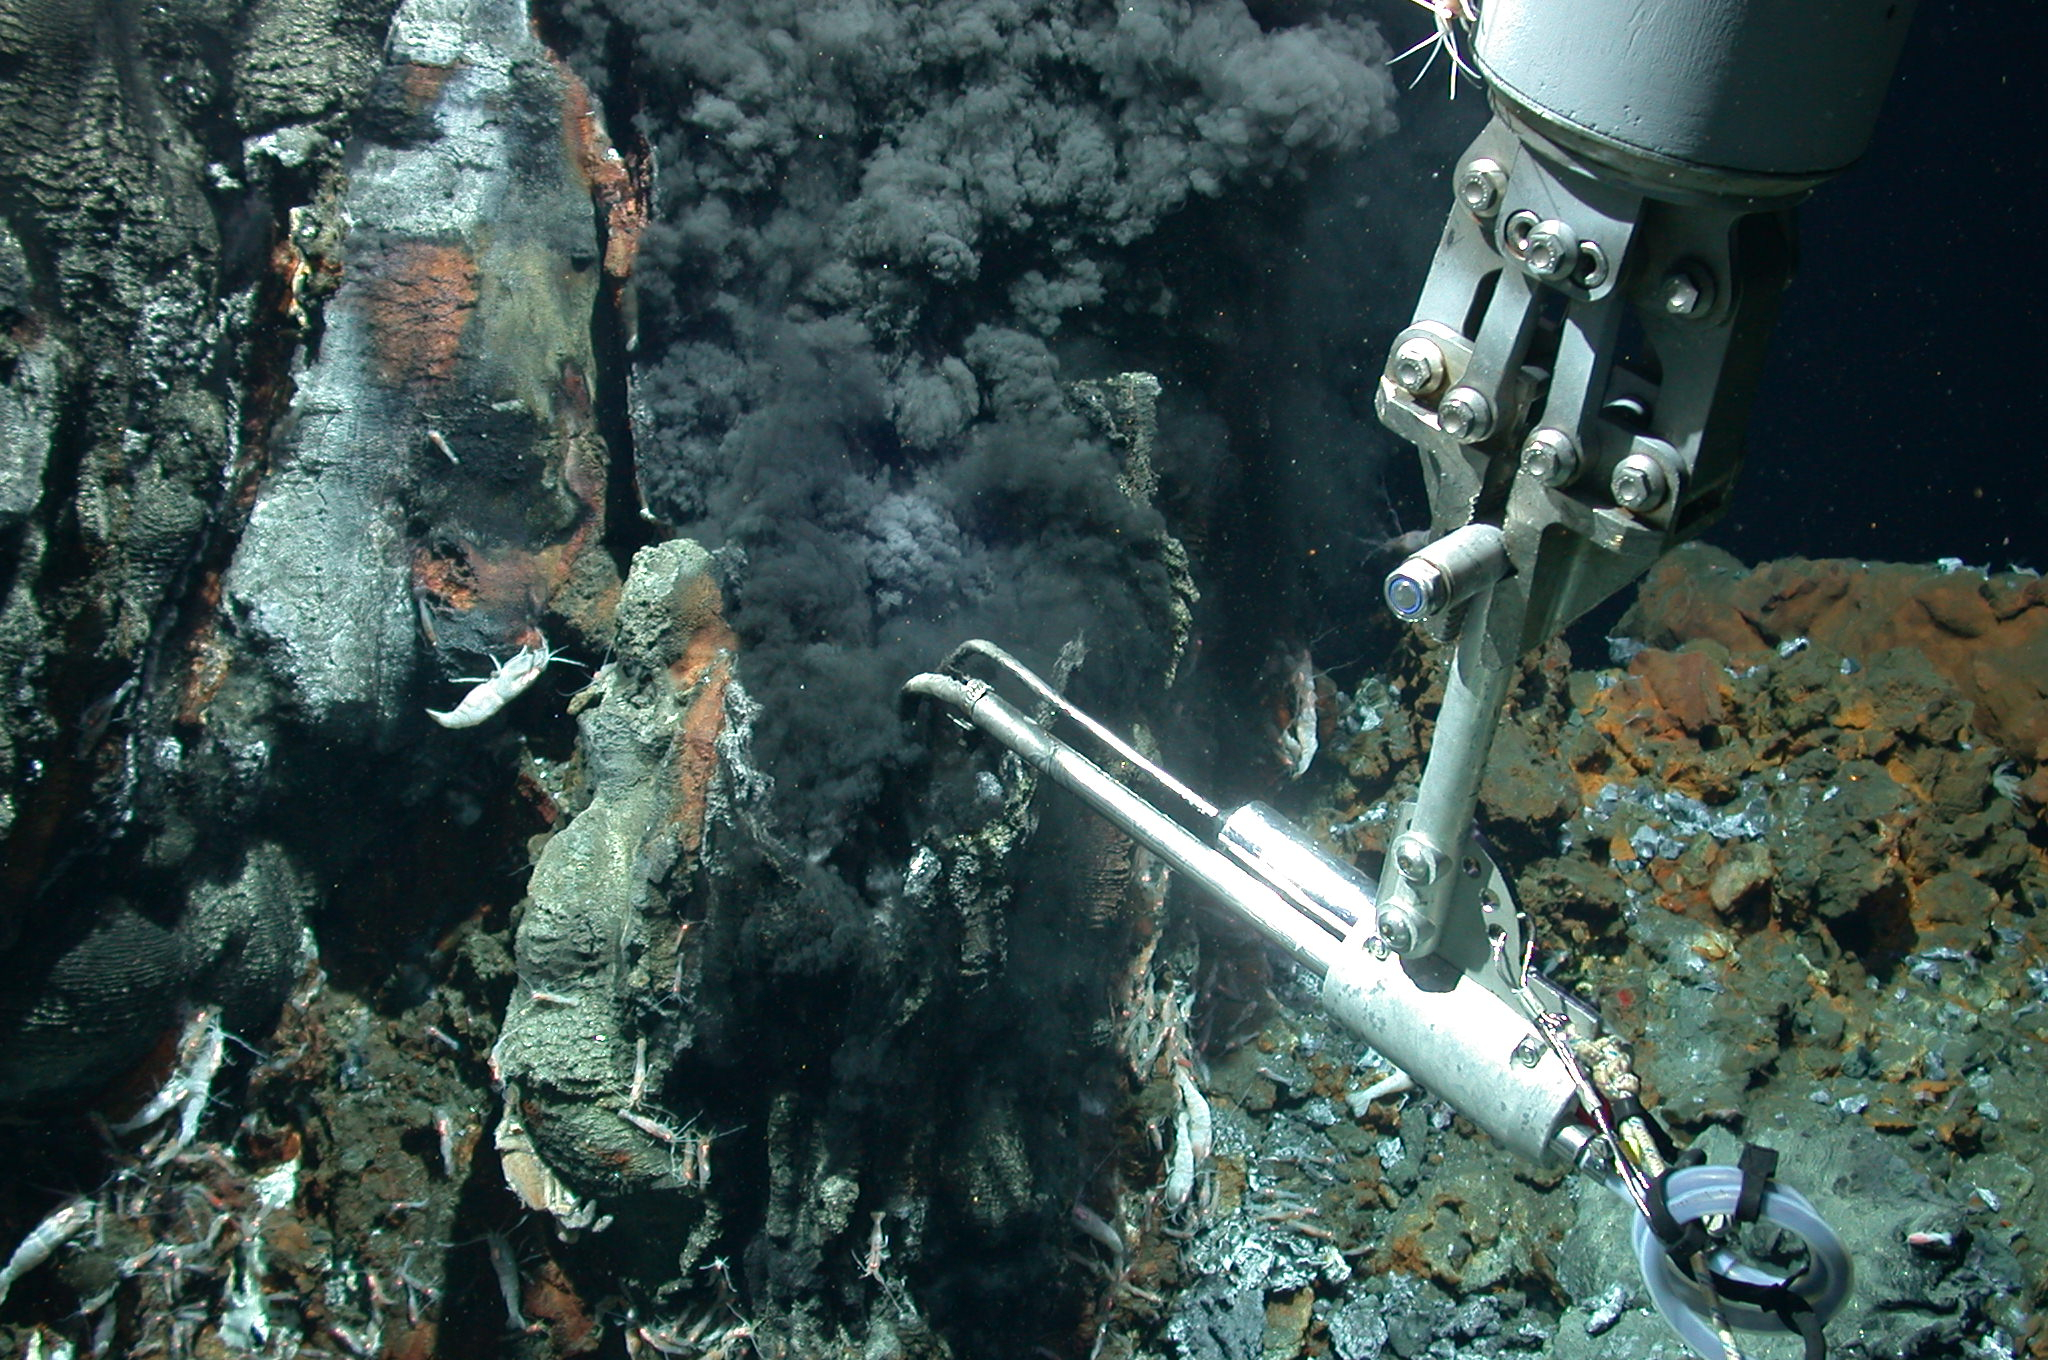
\includegraphics[width=\hsize]{GeoAstro/Koschinsky/Koschinsky_2006_Fig.png}
    \mycaption{Sampling of the hottest hydrothermal vent fluid found so far (407$^\circ$C) at 5$^\circ$S on the Mid-Atlantic Ridge during cruise M68/1. The fluid is taken with the KIPS fluid sampling system equipped with a temperature sensor. (Picture copyright: MARUM, Univ. Bremen)  )}\label{fig:profxxx}
   \end{center}
\end{figure}

\newpage
\paragraph{Collaborations}
\noindent

Regional:
\begin{enumerate}
\item {\sl International University Bremen}\\ Prof. Dr. M. Bau
\item {\sl Universit\"at Kiel}\\Dr. Dieter Garbe-Sch\"onberg
\item {\sl Univ. Hamburg}\\Dr. Richard Seifert
\item {\sl MPI Bremen} \\ Dr. Christian Borowski, Dr. Nicole
Dubilier
\item {\sl BGR Hannover} \\ Dr. Christian Ostertag-Henning, Dr. Thomas
Pletsch, Dr. Thomas Oberth\"ur, BGR
Hannover
\item {\sl Universit\"at Bremen, MARUM}\\ Dr. Volker Ratmeyer, Christian
Seiter
\end{enumerate}

National:
\begin{enumerate}
\item {\sl Univ. M\"unster} \\ Prof. Dr. Harald Strau\ss
\end{enumerate}

International:
\begin{enumerate}
\item {\sl US Geological Survey, Menlo Park, CA}\\ Dr. James Hein
\item {\sl University of Otago, New Zealand}\\ Dr. Sylvia Sander
\item {\sl Universidade de Santa Maria, Brazil} \\ Prof. Dr. Leandro
de Carvalho
\item {\sl Woods Hole Oceanographic Institution, MA}\\ Dr. Chris
German
\end{enumerate}


\paragraph{Grants}
% list the running grants in 2005, if none have been received, please delete this
% subsection.
\begin{enumerate}
\item
Funded by DFG, \emph{Vom Mantel zum Ozean: Stoff-, Engergie- und Lebenszyklen an
  Spreizungsachsen},  KO 2310/2-3,  P.I.: {A.Koschinsky} (November 2005 - July 2008)

\item
Funded by DFG, \emph{Die redoxabh\"angige Fraktionierung von Selen und Tellur in
  geochemischen Systemen\dots}, KO 2906/4-1, P.I.: {A. Koschinsky, } M. Bau, (September
2006 - September 2008)
 
\item
Funded by BGR (Bundesanstalt f\"ur Geowissenschaften und Rohstoffe) Hannover,
\emph{Literaturstudie Manganknollen}, (September 2006 - April 2007)

\item
Funded by DAAD, \emph{PROBRAL exchange program with Brazil. Speciation of
elements of clinical and environmental relevance in saline fluids}, DAAD Project
no. 415-br-PROBRAL/po-D/05/30366, (January 2006 - December 2007)

%\paragraph{References}
%\bibliography{combined}
\end{enumerate}
